%%% fs-seim-stream - Stream processing concepts

%%% TODO: replace event to item
%%% TODO: the/a figure 

\label {fs-stream}

In this section we define some preliminaries for distributed stream processing. It allows us to unify required terms and to introduce definitions, which are needed for the subsequent statements.

In this paper a stream processing system is considered as a shared-nothing distributed runtime. It handles input items and processes them one-by-one according to user-provided logic. It is able to handle a potentially unlimited number of items. The main requirement of this kind of data processing systems is to provide low latency between event occurrence and its processing under fixed load. The term {\em distributed} implies that user's procedures can be partitioned on distinct computational units or shards. The following subsections detail the properties of such systems more precisely.  

\subsection{Data flow}
The basic data flow abstraction is a {\it stream}. The stream is an infinite sequence of data items. Each data item contains a payload defined by a user. Besides, it can be accompanied by meta-information. Typically meta-information is used to define an order on data items. For instance, it can be represented as a UNIX timestamp in milliseconds.

%%% Trace?

\subsection{Computation flow}
Commonly, the computational pipeline is defined in the form of {\it logical graph}. The vertices of the logical graph are operations, and the edges are links between them. Logical graph defines only relations between operations, but it does not describe the physical deployment. The logical graph for the pipeline shown in figure~\ref{break-order-dataflow} is presented in the figure~\ref{break-order-dataflow-logical}

\begin{figure}[htbp]
  \centering
  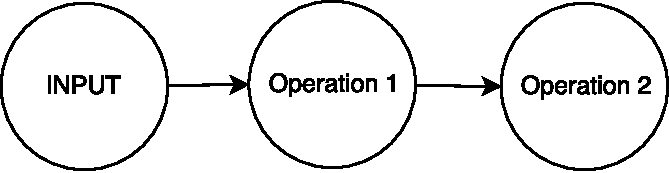
\includegraphics[width=0.38\textwidth]{pics/break_order_pipeline_logical}
  \caption{The logical graph for the physical graph} 
  \label {break-order-dataflow-logical}
\end{figure}

\subsection{Operations}
There are two main types of streaming operations: {\it stateless} and {\it stateful}. Stateless operations do not need any knowledge about past inputs to correctly process current one. A simple illustration is a map operation that multiplies by 2 any numeric input item's payload. On the other hand, stateful operations are able to keep some aggregations or summaries of received events. In such case, the output of the operation depends not only on the input but also on its current state. As an example, one can define an operation that sums all previous items with numerical payloads.

\subsection{Physical deployment}
As mentioned above, each operation can be partitioned between multiple computational units. Data items can be balanced between partitions by key extracted from an item's payload for stateful operations. For stateless operations items can be balanced randomly. The schema of physical partitioning of operations is sometimes called {\it physical graph}. Regarding physical links between operations, in the most cases, it is assumed that they guarantee FIFO order.

\subsection{Guarantees}
Recognized important property of stream processing systems is the type of guarantees it provides in case of failures. There are three main types of such guarantees. {\it At most once} semantics states that each input event is processed once or not processed at all. {\it At least once} guarantees that each input item is processed, but possibly multiple times, that can lead to result duplication. {\it Exactly once} semantics guarantee that each input event is processed exactly one time.  
